\section{Conceptual Framework}

Based on the preliminary results from these studies, we conceived the following themes to make more effective recommendations to software developers.

\subsection{Demonstrate Desire}

In the \peer~study, we found that participants expressing  eagerness  to  use  a  recommended  tool led to more effective recommendations.  For example, during one study session a participant suggested using multi-level sorting functionality in Excel. Their partner demonstrated a desire to use the tool by  responding ``Oh!  Add  level!  Yes, awesome!" and adopted multi-level sorting for the remaininder of the study tasks. This suggests recommending desireable tools and actions can increase adoption among developers. Meanwhile, in another case a participant asked their partner if they wanted to use the R statistical computing software\footnote{https://www.r-project.org/} to complete a task, but their partner responds ``No, no, no...". This shows how a lack of desire to use a specific tool can negatively impact the outcome of a recommendation. 

This idea of using desire in tool recommendations has also been presented in prior work on recommender systems. History-based recommendation systems use past actions by users to measure desire~\cite{Murphy-Hill2012Fluency}. Singer and colleagues studied diffusion of innovations in recommendations and found that the way in which recommendations are communicated impacts desire and reception~\cite{singer2013improving}. Furthermore, Fischer argues recommender systems should actively make suggestions while users are  completing tasks~\cite{FischerActiveHelp}. Goal-recognition techniques such as the  Lumi`ere  Project have been developed to predict desire and anticipate user goals and needs to  effectively recommend useful tools~\cite{horvitz1998lumiere}.

\subsection{Familiarity}

Another key takeaway from the \peer~study is that users are more likely to adopt recommendations for tools and concepts they are familiar with it. In this study, we defined this criteria as users explicitly expressing familiarity with the environment surrounding a recommended tool. An example of an familiarity impacting the outcome of a recommendation in our experiment arose when a participant recommended using R to create a plot for analyzing the data, but their partner responded ``I don’t know R". Even though the recommendation could have been helpful for completing the task, it was ignored because of the recommendee's unfamiliarity with R. Based on these findings, suggesting tools users are familiar with can increase recommendation effectiveness. When recommending new and unfamiliar tools to users, recommendations should have familiar functionality or usage.

Prior work in recommendation systems also suggests familiarity can impact effectiveness. Fogg notes that users are more likely to be receptive to adopting target behaviors if they are familiar with them~\cite{Fogg2009Persuasive}. Murphy-Hill and colleagues propose integrating familiarity into recommender systems by ranking commands based on similarity of those used by colleagues with collaborative filtering.

\subsection{Social Context}

In the results from the \sorry~study, we found that one major issue with our \tele design is its lack of social context. Social context refers to the standard practices and activities necessary to participate in software engineering by interacting with developers and contributing to projects, specifically in open source software. For example, in the \sorry~evaluation many developers complained that \tool did not adhere to formatting guidelines when automatically adding the \EP plugin to project \textit{pom.xml} files. \todo{quotes}.

Prior work also shows that social context is important in making recommendations to software engineers. Johnson and colleagues explored why software engineers don't use static analysis tools and found that the primary reason is the incomprehensible results and feedback from these tools~\cite{Johnson2013Why}. Wessel and colleages studied the usage of software bots in open source software and discovered some of the main challenge developers face during interactions with bots is their poor decision-making and feedback. Furthermore, the top suggested improvements by OSS contributors included making bots smarter and improving interactions with developers~\cite{wessel2018power}.

\subsection{Developer Workflow}

Another key result from \sorry was that the \tele in \tool disrupted the workflow of developers. The most notable example of this was the fact that our automated pull request recommendations of \EP often broke builds for repositories. Many projects have adopted continuous integration systems, such as TravisCI,\footnote{https://travis-ci.org/} to automatically build and integrate changes into projects. However, modifying projects to add a new static analysis tool often introduced many new errors and caused the build to fail. An example of this from our evaluation can be seen in Figure~\ref{fig:error}. Out of the 52 pull requests made, at least 17 resulted in a broken build. This interruption of developer workflow often discouraged users from merging pull requests from our system and accepting the recommendation. \todo{quotes}

Prior work in software engineering also notes the importance of integration into the workflow of developers. Johnson and colleagues also discovered that software engineers avoid static analysis tools because they lack customizability and are difficult to integrate into the development process~\cite{Johnson2013Why}. To improve  recommendations, bots  should  suggest  tools without breaking existing infrastructure.  One solution is to change how  potential  users  interact  with  tools.  For instance, rather than fully integrating tools with automated pull requests, allow developers to incrementally use them, i.e., modifying the \EP plugin to report errors as warnings instead of compilation errors or implementing a demo-mode for users to try  the tool in a sandbox environment without impacting builds. Another solution is to help developers further by fixing issues introduced  in  the  build. For instance, the program repair bot  Repairnator presents developers with patches for errors~\cite{Repairnator}. Automatically  fixing  reported  bugs  can  improverecommendations within developer workflows.

% %This section presents approaches for making recommendations to developers. These designs are derived from prior work in peer interactions and concepts from nudge theory, and differ on the locality and actionability of the suggestions. Our conceptual framework introduces novel digital nudges types for making recommendations to software engineers: \telemarketer; \location; and \timing. Each of these constituted nudge types are defined and motivated below. This research aims to evaluate the effectiveness of the conceptual framework in increasing software engineering action adoption among developers by building tools and examining existing systems that implement these digital nudge types.d

% %\subsection{\location}

% To examine the effectiveness of spatial locality for digital nudges, we came up with \textit{situated nudges}. Situated nudges make suggestions to software developers at the location where a useful software engineering action is applicable.

% High spatial locality

% %\subsection{\timing}

% Location (hot and cold) [nudge theory] finds that timely feedback can improve acceptance of suggestion. Examples of these in real life? For example, handing out floss, right before entering a bathroom after eating ribs, increased chances of adopting flossing by 20\% (\todo{replace with example not completely made up}).

% To evaluate the timing of digital nudges, we introduce the concept of \emph{just-in-time nudges}. These nudges make recommendations to developers at a moment when a software engineering action is appropriate.

% We hypothesize that developers will prefer just-in-time nudges when a software engineering tool is most applicable over nudges presented at different times. Recommendations made when they are appropriate provide more convenience to users so developers don't have to figure out when's the best time to use a tool or practice. This can help improve adoption of software engineering actions for developers while they are completing programming tasks. A potential downside to just-in-time nudges is that they can interrupt developers in their work, which research suggests may lead to a loss of task context~\cite{parnin2010interrupted}.

% High temporal locality

\begin{figure*}
\centering
	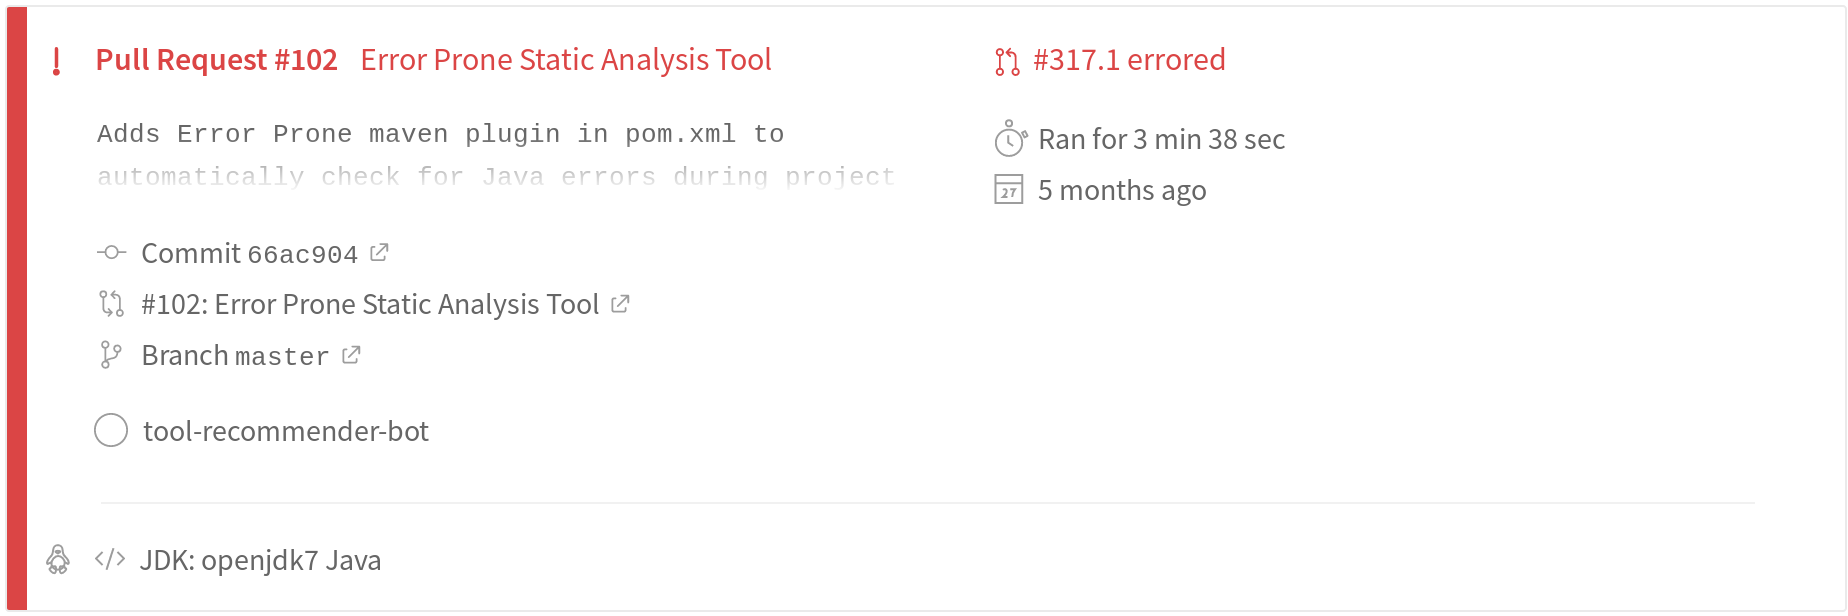
\includegraphics[width=\textwidth]{images/error.png}
	\caption{Example of an automated pull request from \tool causing a project build to fail}	
	\label{fig:error} 
\end{figure*}


% %\subsection{Public nudge}

% %Humans are more likely to adopt behavior if there is external pressure to do so.

% %We define \textit{public nudges} as nudges that are visible and available to see by a specific community. They may also involve social pressure if certain behaviors aren't adopted. For example, badges on GitHub are public nudges viewable to users who visit a repository and can influence their decision to contribute or use the product. These badges display whether projects adopt certain software engineering behaviors, such as passing builds. Figure \ref{fig:red_badge} presents a badge for a project that does not use a useful software engineering processes during development, while the developers for a project with a badge in Figure \ref{fig:green_badge} integrate software engineering actions in their development process. Trockman and colleagues examined the effect of these public nudges for npm\footnote{https://www.npmjs.com/} packages on GitHub and found that the addition of badges correlated with improvements in the quality of the project, i.e. adding a quality assurance badge displaying code coverage increased the coverage of tests~\cite{trockman2018badges}

% %Our hypothesis is that developers are more likely to adopt useful software engineering actions if they are publicly nudged to do so.

% % \begin{figure}
% % \centering
% % \subfigure[Project without a software engineering action]{
% % \label{fig:red_badge}
% % 
\includegraphics[width=\textwidth/2]{images/badge1.png}}
% % \qquad
% % \subfigure[Project with a software engineering action]{
% % \label{fig:green_badge}
% % 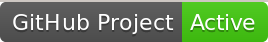
\includegraphics[width=\textwidth/2]{images/badge2.png}}
% % \caption{Example of a public nudge}
% % \end{figure}

% % [benefits/trade-offs;hypothesis]

% % \subsection{Social nudge}

% % Nudge theory finds that people are more likely to adopt a useful behavior if others they know already do it. Perloff studied the impact of social media on body image and self-perception among American girls, and proposes using ``media-based interventions...to nudge individuals into changing their attitudes and behaviors"~\cite[p.~364]{perloff2014social}. This work suggests social media use is key in creating social comparisons and influencing users to adopt harmful behaviors such as body dissatisfaction and eating disorders.

% % To study digital nudges in a social context, we introduce \textit{social nudges}. These nudges suggest software engineering actions that have been adopted by a developer's friends or colleagues. An example of this is seen in prior work examining peer interactions. Murphy-Hill conducted interviews and surveys with software engineers and found that developers prefer recommendations from peers over other methods of tool discovery such as tutorials, discussion threads, tool encounters, and written descriptions~\cite{Murphy-Hill2015HowDoUsers}.

% % Our hypothesis is that developers are more likely to adopt behaviors recommended in a nudge if they know it is used by a friend or colleague.

% % \subsection{Apprehensive nudge}

% % If you can show a target behaviors usefulness by presenting multiple places it can be applied, people are more likely to adopt it.

% % We created the concept of \textit{apprehensive nudges}, which provide multiple locations where software engineering activities can be applied, to study how this impacts activity adoption for developers.

% % [Conceptual implementation]

% % [benefits/trade-offs;hypothesis]

% % \subsection{Automated nudge}

% % If you do the work for them, humans are more likely to adopt specific behaviors. \todo{Example= automatic magazine subscription renewal due to status quo bias [Nudge, 35]}

% % To determine if automatically performing software engineering actions for developers impacts adoption for developers, we introduce \textit{automated nudges}. There are many ways automation is used to improve software engineering and help developers adopt helpful behaviors. For instance, Mirhosseini and colleagues investigated creating automated pull requests to convince developers to upgrade outdated dependencies using greenkeeper\footnote{https://greenkeeper.io} to manage dependency package versions for GitHub projects~\cite{sam2017autopullrequests}. They found that automated pull requests were useful in increasing awareness of out-of-date package dependencies to developers.

% % [benefits/trade-offs;hypothesis]

% % \subsection{Tutorial nudge}

% % If you show people how to do a certain behavior, then they are more likely to adopt it.

% % We define \textit{tutorial nudges} as digital nudges that show developers how to use a specific software engineering tool or programming activity. For example,...

% % [Conceptual implementation]

% % [benefits/trade-offs;hypothesis]

% % \subsection{Reminder nudge}

% % If you continually remind humans to adopt a certain activity, they are more likely to adopt it.

% % To evaluate the effectiveness of reminders, we developed \textit{reminder nudges} to periodically recommend useful software engineering actions to programmers.

% % [Conceptual implementation]

% % [benefits/trade-offs;hypothesis]

% % \subsection{Positive nudge}

% % Nudge theory suggests using positive language is more effective in helping people adopt target behaviors. For example, Doberstein and colleagues evaluated using positive messages to improve attitudes about increasing residential housing density in Canada~\cite{doberstein2016positive}. They compared a neutral control statement of benefits with public statements, private statements, and expert comparisons.  \todo{Framing [Nudge, 36-37]}

% % To determine if developers respond better to positive or negative recommendations, we introduce \textit{positive nudges} that commend developers for their work rather than blaming them to encourage future software engineering action adoption.

% % If you recommend developer actions in a positive way, then developers are more likely to adopt them.

% % \subsection{Effects}

% % We hope our nudges have some of the following effects on developers who receive recommendations for software engineering actions...

% % \todo{Some interesting effects to consider:}
% % \begin{itemize}
% % \item Baader-Meinhof --- you start seeing something you just learned or on your mind everywhere.
% % \item Diderot Effect --- the act of getting one new thing triggers a cascade of other new things.
% % \item Novelty Effect --- using something new makes you think you are more productivity
% % \item ... should look at behavioral and marketing psychology stuff...
% % \end{itemize}
